\documentclass[12pt]{article}
\usepackage[utf8]{inputenc}
\usepackage{graphicx} % Allows you to insert figures
\usepackage{amsmath} % Allows you to do equations
\usepackage{fancyhdr} % Formats the header
\usepackage{geometry} % Formats the paper size, orientation, and margins
\usepackage[style=authoryear-ibid,backend=biber]{biblatex} % Allows you to do citations - does Harvard style and compatible with Zotero
\addbibresource{Example.bib} % Tells LaTeX where the citations are coming from. This is imported from Zotero
\usepackage[english]{babel}
\usepackage{csquotes}
\usepackage{background}
\usepackage{minted}
\renewcommand*{\nameyeardelim}{\addcomma\space} % Adds comma in in-text citations
\linespread{1.5} % About 1.5 spacing in Word
\setlength{\parindent}{0pt} % No paragraph indents
\setlength{\parskip}{1em} % Paragraphs separated by one line
\renewcommand{\headrulewidth}{0pt} % Removes line in header
\geometry{a4paper, portrait, margin=1in}
\setlength{\headheight}{14.49998pt}
\backgroundsetup{scale=1,angle=0,opacity=0.175,contents={
\includegraphics[scale=0.25]{1200px-Vellore_Institute_of_Technology_seal_2017.png}}}


\begin{document}
\begin{titlepage}
\NoBgThispage
   \begin{center}
        \begin{figure}[h] % h - Place the float here, i.e., approximately at the same point it occurs in the source text (however, not exactly at the spot)
        \centering
        
\includegraphics[width=15cm]{1583124354phpJTtnK5.png}
        \end{figure}

        \Huge{Digital Assignment 2}

        \vspace{0.5cm}
        \LARGE{20BIT0380 - Hardik Nagpal\\20BIT0386 - Raghav Gupta\\20BIT0381 - Niladri Mitra\\20BIT0406 - Sanchit Sandeep Khedkar\\20BIT0015 - Atishay Jain}
       
        \vspace{2.5 cm}

        \vspace{0.25 cm}
        \Large{ITE2015 - Information Systems Audit}
        \large{VL2021220502557}
       

       \vfill
    \end{center}
\end{titlepage}
\newpage
Q1. Mention the key management practices which are required for aligning IT strategy with enterprise strategy which can be measured by evaluating the benefits realised from IT enabled investments and services.
\par
Ans- \\
In an ideal universe, the IT and enterprise worlds would be perfectly aligned, with IT supplying enterprise leaders with the strategic plans and resources necessary to achieve maximum performance, efficiency and profits. Yet, as you may have noticed, seeking perfection can be a somewhat elusive quest. In the real world, IT leaders are often left guessing whether the plans they’ve created and the technologies they’ve selected are actually fulfilling enterprise expectations. Enterprise leaders, meanwhile, frequently fret that IT isn’t fully tuned in to actual enterprise needs and challenges. Today, most of the organizations depended on the IT and have a high investment in IT infrastructures and initiatives to get in line with market innovations and digital transformations. All departments, roles, and enterprise levels are supported by IT. IT is central to organizational success – effective and efficient delivery of services and goods – especially when the IT is designed to bring about digital transformation or enterprise transformation. The innovation and digital transformation are a challenge for organizations, a disruptive attitude offers many rewards and competitive advantages, but it is synonymy of risks and unintended consequences. Also, the market and regulations exigences, like to protection of confidential information, financial accountability, data retention and disaster recovery, and among others, are a pressure factor for organizations that require a high control of internal and external information, and the IT support. Fortunately, there are proven methods that enable IT leaders to gain a clear understanding of the IT-enterprise relationship. The following seven suggestions show how to build a productive partnership that will satisfy stakeholders’ needs while meeting IT’s time and budget constraints.
\\
1. Build close enterprise relationships: Whether face-to-face or Zoom-to-Zoom, IT leaders should set aside time to meet and discuss important matters with enterprise leaders across their enterprise. “A key component to a good dialogue is simply to speak in plain English, even when trying to explain complex technical issues,” advises Nidal Haddad, principal for ecosystems and alliances at enterprise advisory firm Deloitte Consulting. Building close alignment between IT and enterprise requires committing to earnest, insightful discussions. Imagine, for instance, a conversation about AI. In this example, the enterprise leader wants to adopt the technology, but doesn’t understand that AI is primarily cloud-based or that AI works best when fueled by large amounts of data. “By explaining the concepts behind AI in a clear manner, the enterprise leader can be introduced to the building blocks for AI, and the IT leader can develop an acceptable strategy,”. To build strong, close ties, IT management also needs to listen to and learn from their enterprise counterparts. “IT leaders can’t create a plan to enable enterprise priorities in a vacuum,” . “It’s better to ask [enterprise] leaders to share their plans, removing the guesswork around enterprise needs and intentions.” Remember, too, that IT is a key player in defining the corporate vision. “Most successful IT departments serve as powerful enablers, magnifying the strategy of the enterprise and compounding its success”.
\\
A close interpersonal relationship is powerful because it “gut checks IT initiatives against enterprise growth plans,”. “IT folks shouldn’t be afraid to reach out to their colleagues, whether in marketing, accounting or any other department, to better understand their pain points and to brainstorm solutions together,”, noting that collaboration tools, such as Slack, are “invaluable in maintaining a free and open dialogue.”
\\
2. Ask the right questions: When meeting with enterprise colleagues, it’s natural to zero in on questions relating to IT technologies, strategies and operations. Yet these topics are a strange, foreign territory for most enterprise leaders. “It requires them to role-play your job, and they’re not very good at that because it’s never been their job,”. Its far more useful and productive to ask enterprise leaders about their own jobs, including their view of market trends and the key enterprise challenges they’re facing. “It’s then our job on the IT side to evaluate where technology solutions could be brought online to service those needs,”. “That’s really the essence of the IT mission statement.”
\\
3. Build trust: Successful relationships are built on trust, transparency, mutual respect and shared goals. Professional connections are no different. “Ensuring you have a deep understanding of your partners’ enterprise, taking extreme ownership of challenges and being vulnerable are all tenants of building tight partnerships,” observes Andrew Palmer, CIO for the U.S. Region at Liberty Mutual Insurance.\\
Failing to align IT and enterprise interests gradually erodes hard-earned trust. “It fuels skepticism in technology strategies, promotes a culture of blame, reduces patience and forces planning into unproductive levels of detail resulting in a false sense of precision,” . When enterprise leaders have confidence in their IT organization, everything moves faster. “Decision-making is crisper, risk-taking is increased and teams spend more time executing than planning.” Creating and cultivating a culture that supports constant, open communication is another key to building close and trusting IT and enterprise collaboration. “The result is one team with shared goals and objectives,” managing director for global IT and enterprise architecture at enterprise consulting firm Accenture. IT leaders should invite enterprise leaders to discuss the challenges and goals of day-to-day enterprise processes and how IT can help improve speed, efficiency and innovation. “This two-way communication culture and encouraging feedback … can let both IT and the enterprise know how to continue improving collaboration,”.
\\
4. Become a motivator: Most enterprise leaders expect IT to be the engine that propels enterprise success. “Only aiming to meet defined enterprise needs is selling IT short,”. “The best IT teams in the world bring forth their own innovation to solve enterprise needs”. Understand that enterprise leaders may not yet be aware of important new or enhanced technologies. It’s an IT leader’s responsibility, to alert enterprise colleagues to disruptive and transformational technologies with the potential to change the entire enterprise landscape, as well as lesser innovations that can lead to incremental market and performance enhancements
\\
5. Learn from surveys: Surveys should be designed with the goal of providing deep insights into the overall enterprise vision, including strategy, key priorities and required capabilities. IT surveys have traditionally focused on technology and service quality in areas such as help desk support, delivery reliability, systems stability and security, Palmer notes. Times have changed, however. A modern survey should target the ways IT can help drive the enterprise vision. “The goal is to capture the outcomes required to win around the core strategy, such as growth, profit, customer experience and innovation”.
\\
Survey questions will vary, depending on the target responders. “The key is to create surveys that are short and allow flexibility with answers,”. “Qualitative feedback is just as importance as the percentages”.
\\
6. Conduct ongoing assessments: Like any enterprise optimization initiative, IT/enterprise alignment should be viewed as an open-ended project. “Establish processes to ensure redundancy and oversight to determine whether the relationship is successful or needs improvement,” “It’s really about constantly and consistently maintaining a dialogue with counterparts across the company,”. Assessing alignment should be a constant conversation within IT management. “With consistent and frequent alignment checks, the IT team will evolve from being reactive to being proactive,”. “A proactive IT team works to fix and address issues before they occur rather than waiting for a problem to force damage control and recovery.”
\par
Q2. In the auditing process, when auditors evaluate application systems, why do they focus on controls over classes of transactions rather than on individual transactions? Explain.
\par
Ans-\\
In some organizations, strategic information systems planning is a critical function, but in others it has only minor importance. Auditors must be knowledgeable and astute in determining the ways that management functions should be performed in each organization evaluated. Otherwise, judgments on what events are lawful will be misguided.
\\
As a basis for identifying Lawful and unlawful events in application subsystems, we focus on the transactions that can occur as input to the subsystem. All events in an application system must arise from a transaction. The application system initially changes state can event occurs when the transaction is first received as an input. For example, an order-entry system must record an order when it is first entered into the system. Further state changes (events) then occur as the application system processes the transaction. For example, after an order-entry system has stored an open order, it then attempts to fill the order. Lawful events will arise if the transaction and subsequent processing are authorized, accurate, complete, nonredundant, effective, and efficient. Otherwise, unlawful events will occur.
\\
To identify all the events that might arise in an application system as a result of a transaction, we must understand how the system is likely to process the transaction. Historically, auditors have used walk-through techniques to accomplish this objective: They consider a particular transaction, identify the particular components in the system that process the transaction, and then try to understand each processing step that each component executes. They also consider any errors or irregularities (unlawful events that might occur along the way. For example, auditors might focus on a credit sale transaction. After the transaction has been entered into the sales system, they would trace the credit sale through each processing step executed by the order-entry program. They would also consider how the transaction might be entered improperly and how subsequent processing errors or irregularities might arise.
\\
It is often costly to trace each individual transaction through an application system to obtain an understanding of all the different types of events that can occur in the system. For this reason, auditors sometimes focus on classes of transactions. In other words, they group transactions together in the transactions undergo similar processing. They then try to understand these transactions and the events that arise as a result of these transactions as a group. In addition, they focus only on those transactions they consider to be material from the viewpoint of their audit objectives. Using these strategies, not all events that can occur in a system are identified. Nevertheless, auditors should examine all those transactions and events that they consider to be important.
\\
When the material events that can occur in a management of application system have been identified, auditors must evaluate whether controls are in place and working to cover the unlawful events. Accordingly, they collect evidence on the existence and reliability of controls to determine whether expected losses from unlawful events have been reduced to an acceptable level. They consider each type of unlawful event that might arise, whether controls cover each of these events, how reliable these controls are, and whether a material error or irregularity can still occur. Lists have been published to assist with this task showing failings that occur in management subsystems and errors and irregularities that occur for different types of transactions in different types of applications systems. These lists also show various controls that can be used to reduce expected losses from these errors and irregularities. Table below is an example of one such list for a customer order transaction in an order-entry application system.
\\
\begin{figure}[h] % h - Place the float here, i.e., approximately at the same point it occurs in the source text (however, not exactly at the spot)
\centering
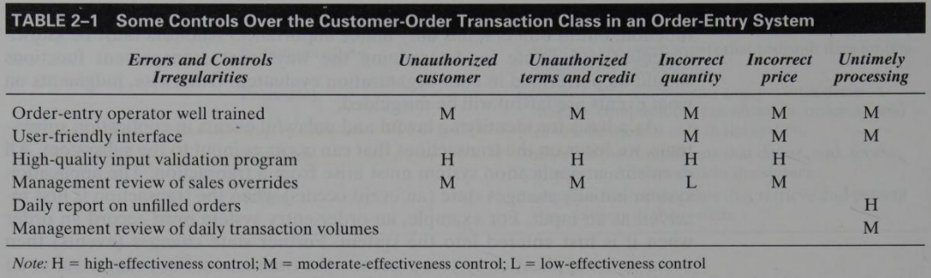
\includegraphics[\textwidth]{Screenshot 2022-04-26 160157.png}
\end{figure}
\newpage
The table shows a controls matrix in which the columns show errors or irregularities that can occur and the rows show controls that can be set up to reduce expected losses from these errors and irregularities. The elements of the matrix show an auditor's assessment of how effective each control is in reducing expected losses from each type of error or irregularity. For every system at every level in the level structure, the evaluation steps are the same. The transactions that might enter the system are first identified. The lawful and unlawful events that can occur as a result are then considered. Finally, the reliability of the controls that cover the unlawful events is assessed. As we evaluate higher-level systems, we are likely to encounter new controls for three reasons. 
\\
First, controls in lower-level systems can malfunction. Recall, a control is a system itself, and it can be unreliable like any other system. A higher-level control might be implemented to cover unlawful events that arise when lower-level controls fail to prevent, detect, or correct them. For example, consider a group of clerks that process mail orders. Work might be divided among them based on the first letter of customers' surnames. Thus, several subsystems exist to process orders from different groups of customers. Each clerk might exercise certain controls to prevent, detect, or correct errors. Nevertheless, their manager might also examine the quality of their work. Managers are responsible for the quality of work in all subsystems, and they are exercising a higher-level control in case a lower-level control malfunction.
\\
Second, it might be more cost-effective to implement controls at higher levels. Again, consider our example of the group of clerks who process mail orders. If they are well trained and diligent, they might not be required to double-check! their work. Given the low error rate that is expected to occur, the cost of doublechecking might be too high. Their manager periodically might take a sample of their work, however, to assess its quality. The higher-level control is more cost-effective because it is exercised by one person who has greater facility with the control rather than multiple persons, each of whom has less facility with the control
\\
Third, some events are not manifested as unlawful except in higher level systems. For example, an employee might query a database to obtain the average salary of female consultants employed within an organization. The sub-system that processes the query might deem this query to be a lawful event.
\end{document}
